\documentclass[11pt,]{article}
\usepackage{lmodern}
\usepackage{amssymb,amsmath}
\usepackage{ifxetex,ifluatex}
\usepackage{fixltx2e} % provides \textsubscript
\ifnum 0\ifxetex 1\fi\ifluatex 1\fi=0 % if pdftex
  \usepackage[T1]{fontenc}
  \usepackage[utf8]{inputenc}
\else % if luatex or xelatex
  \ifxetex
    \usepackage{mathspec}
  \else
    \usepackage{fontspec}
  \fi
  \defaultfontfeatures{Ligatures=TeX,Scale=MatchLowercase}
\fi
% use upquote if available, for straight quotes in verbatim environments
\IfFileExists{upquote.sty}{\usepackage{upquote}}{}
% use microtype if available
\IfFileExists{microtype.sty}{%
\usepackage{microtype}
\UseMicrotypeSet[protrusion]{basicmath} % disable protrusion for tt fonts
}{}
\usepackage[margin = 1.5in]{geometry}
\usepackage{hyperref}
\PassOptionsToPackage{usenames,dvipsnames}{color} % color is loaded by hyperref
\hypersetup{unicode=true,
            pdftitle={Financial Time Series},
            pdfauthor={Abhinav Anand, IIMB},
            colorlinks=true,
            linkcolor=blue,
            citecolor=magenta,
            urlcolor=red,
            breaklinks=true}
\urlstyle{same}  % don't use monospace font for urls
\usepackage{color}
\usepackage{fancyvrb}
\newcommand{\VerbBar}{|}
\newcommand{\VERB}{\Verb[commandchars=\\\{\}]}
\DefineVerbatimEnvironment{Highlighting}{Verbatim}{commandchars=\\\{\}}
% Add ',fontsize=\small' for more characters per line
\usepackage{framed}
\definecolor{shadecolor}{RGB}{248,248,248}
\newenvironment{Shaded}{\begin{snugshade}}{\end{snugshade}}
\newcommand{\KeywordTok}[1]{\textcolor[rgb]{0.13,0.29,0.53}{\textbf{#1}}}
\newcommand{\DataTypeTok}[1]{\textcolor[rgb]{0.13,0.29,0.53}{#1}}
\newcommand{\DecValTok}[1]{\textcolor[rgb]{0.00,0.00,0.81}{#1}}
\newcommand{\BaseNTok}[1]{\textcolor[rgb]{0.00,0.00,0.81}{#1}}
\newcommand{\FloatTok}[1]{\textcolor[rgb]{0.00,0.00,0.81}{#1}}
\newcommand{\ConstantTok}[1]{\textcolor[rgb]{0.00,0.00,0.00}{#1}}
\newcommand{\CharTok}[1]{\textcolor[rgb]{0.31,0.60,0.02}{#1}}
\newcommand{\SpecialCharTok}[1]{\textcolor[rgb]{0.00,0.00,0.00}{#1}}
\newcommand{\StringTok}[1]{\textcolor[rgb]{0.31,0.60,0.02}{#1}}
\newcommand{\VerbatimStringTok}[1]{\textcolor[rgb]{0.31,0.60,0.02}{#1}}
\newcommand{\SpecialStringTok}[1]{\textcolor[rgb]{0.31,0.60,0.02}{#1}}
\newcommand{\ImportTok}[1]{#1}
\newcommand{\CommentTok}[1]{\textcolor[rgb]{0.56,0.35,0.01}{\textit{#1}}}
\newcommand{\DocumentationTok}[1]{\textcolor[rgb]{0.56,0.35,0.01}{\textbf{\textit{#1}}}}
\newcommand{\AnnotationTok}[1]{\textcolor[rgb]{0.56,0.35,0.01}{\textbf{\textit{#1}}}}
\newcommand{\CommentVarTok}[1]{\textcolor[rgb]{0.56,0.35,0.01}{\textbf{\textit{#1}}}}
\newcommand{\OtherTok}[1]{\textcolor[rgb]{0.56,0.35,0.01}{#1}}
\newcommand{\FunctionTok}[1]{\textcolor[rgb]{0.00,0.00,0.00}{#1}}
\newcommand{\VariableTok}[1]{\textcolor[rgb]{0.00,0.00,0.00}{#1}}
\newcommand{\ControlFlowTok}[1]{\textcolor[rgb]{0.13,0.29,0.53}{\textbf{#1}}}
\newcommand{\OperatorTok}[1]{\textcolor[rgb]{0.81,0.36,0.00}{\textbf{#1}}}
\newcommand{\BuiltInTok}[1]{#1}
\newcommand{\ExtensionTok}[1]{#1}
\newcommand{\PreprocessorTok}[1]{\textcolor[rgb]{0.56,0.35,0.01}{\textit{#1}}}
\newcommand{\AttributeTok}[1]{\textcolor[rgb]{0.77,0.63,0.00}{#1}}
\newcommand{\RegionMarkerTok}[1]{#1}
\newcommand{\InformationTok}[1]{\textcolor[rgb]{0.56,0.35,0.01}{\textbf{\textit{#1}}}}
\newcommand{\WarningTok}[1]{\textcolor[rgb]{0.56,0.35,0.01}{\textbf{\textit{#1}}}}
\newcommand{\AlertTok}[1]{\textcolor[rgb]{0.94,0.16,0.16}{#1}}
\newcommand{\ErrorTok}[1]{\textcolor[rgb]{0.64,0.00,0.00}{\textbf{#1}}}
\newcommand{\NormalTok}[1]{#1}
\usepackage{longtable,booktabs}
\usepackage{graphicx,grffile}
\makeatletter
\def\maxwidth{\ifdim\Gin@nat@width>\linewidth\linewidth\else\Gin@nat@width\fi}
\def\maxheight{\ifdim\Gin@nat@height>\textheight\textheight\else\Gin@nat@height\fi}
\makeatother
% Scale images if necessary, so that they will not overflow the page
% margins by default, and it is still possible to overwrite the defaults
% using explicit options in \includegraphics[width, height, ...]{}
\setkeys{Gin}{width=\maxwidth,height=\maxheight,keepaspectratio}
\IfFileExists{parskip.sty}{%
\usepackage{parskip}
}{% else
\setlength{\parindent}{0pt}
\setlength{\parskip}{6pt plus 2pt minus 1pt}
}
\setlength{\emergencystretch}{3em}  % prevent overfull lines
\providecommand{\tightlist}{%
  \setlength{\itemsep}{0pt}\setlength{\parskip}{0pt}}
\setcounter{secnumdepth}{0}
% Redefines (sub)paragraphs to behave more like sections
\ifx\paragraph\undefined\else
\let\oldparagraph\paragraph
\renewcommand{\paragraph}[1]{\oldparagraph{#1}\mbox{}}
\fi
\ifx\subparagraph\undefined\else
\let\oldsubparagraph\subparagraph
\renewcommand{\subparagraph}[1]{\oldsubparagraph{#1}\mbox{}}
\fi

%%% Use protect on footnotes to avoid problems with footnotes in titles
\let\rmarkdownfootnote\footnote%
\def\footnote{\protect\rmarkdownfootnote}

%%% Change title format to be more compact
\usepackage{titling}

% Create subtitle command for use in maketitle
\newcommand{\subtitle}[1]{
  \posttitle{
    \begin{center}\large#1\end{center}
    }
}

\setlength{\droptitle}{-2em}

  \title{Financial Time Series}
    \pretitle{\vspace{\droptitle}\centering\huge}
  \posttitle{\par}
    \author{Abhinav Anand, IIMB}
    \preauthor{\centering\large\emph}
  \postauthor{\par}
      \predate{\centering\large\emph}
  \postdate{\par}
    \date{2018/07/23}

\linespread{1.25}
\usepackage{amsmath}

\begin{document}
\maketitle

\section{Background}\label{background}

Financial prices, indices, returns etc. are sequences of real numbers
indexed by time. The study of their mathematical and statistical
properties is vital for those aspiring to write papers in empirical
finance.

For example, consider the following plot of a hypothetical market index:
what can we say about the market conditions from its ups and downs?

\begin{center}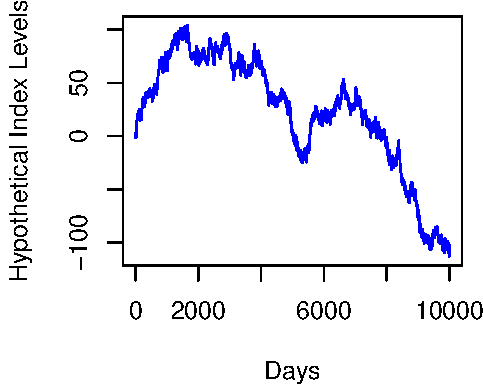
\includegraphics{FMC_T4_PhD_Fin_Time_Series_files/figure-latex/hypo_market_index-1} \end{center}

The above series is, however generated via the command:
\texttt{plot(cumsum(rnorm(10000,\ 0,\ 1))} which plots the cumulative
sum of ten thousand standard normal realizations---a random walk!

The \emph{random walk hypothesis} is a theory that claims that stock
market prices obey a random walk process. This hypothesis is consistent
with the ``Efficient Market Hypothesis''. Roughly speaking, the
efficient market hypothesis claims in its weak form that for publicly
traded stocks, all public information is captured in the price of the
stock. The strong form of the hypothesis claims that \emph{all}
information---both public and private---is reflected the stock price.
Hence according to this theory, any attempt to consistently beat the
market in terms of risk-adjusted returns is doomed to failure.\footnote{Or,
  in other words, if investors beat the market it's not perhaps due to
  their so-called investing skills but due to their being lucky.}

Hence in particular, any attempt to discern patterns in the hypothetical
market's ups and downs as shown above is worthless.

Do empirical financial markets behave in the same way too?

\section{Empirical Financial Time
Series}\label{empirical-financial-time-series}

As an illustration we produce the daily time series for the closing
value of the Bombay Stock Exchange index (``Sensex'').

\begin{Shaded}
\begin{Highlighting}[]
\NormalTok{file_bse <-}\StringTok{ "SENSEX.csv"}
\NormalTok{index_bse <-}\StringTok{ }\NormalTok{readr}\OperatorTok{::}\KeywordTok{read_csv}\NormalTok{(file_bse) }\OperatorTok
\StringTok{  }\NormalTok{dplyr}\OperatorTok{::}\KeywordTok{select}\NormalTok{(}\OperatorTok{-}\NormalTok{empty)}
\NormalTok{index_bse}\OperatorTok{$}\NormalTok{Date <-}\StringTok{ }\KeywordTok{as.Date}\NormalTok{(index_bse}\OperatorTok{$}\NormalTok{Date, }
                          \DataTypeTok{format =} \StringTok{"%d-%B-%Y"}
\NormalTok{                          ) }\CommentTok{#date reformat}

\KeywordTok{plot}\NormalTok{(index_bse}\OperatorTok{$}\NormalTok{Date,}
\NormalTok{     index_bse}\OperatorTok{$}\NormalTok{Close,}
     \DataTypeTok{type =} \StringTok{"l"}\NormalTok{,}
     \DataTypeTok{col =} \StringTok{"blue"}\NormalTok{,}
     \DataTypeTok{xlab =} \StringTok{"Year"}\NormalTok{,}
     \DataTypeTok{ylab =} \StringTok{"BSE Index"}\NormalTok{,}
     \DataTypeTok{main =} \StringTok{"Indian stock market performance"}
\NormalTok{     )}
\NormalTok{fit_lm <-}\StringTok{ }\KeywordTok{lm}\NormalTok{(Close }\OperatorTok{~}\StringTok{ }\NormalTok{Date, }
             \DataTypeTok{data =}\NormalTok{ index_bse) }\CommentTok{#fit linear model}
\KeywordTok{abline}\NormalTok{(fit_lm, }\CommentTok{#plot linear model line}
       \DataTypeTok{lty =} \StringTok{"dotdash"}\NormalTok{, }
       \DataTypeTok{col =} \StringTok{"red"}\NormalTok{,}
       \DataTypeTok{lwd =} \DecValTok{2}
\NormalTok{       )}
\end{Highlighting}
\end{Shaded}

\begin{center}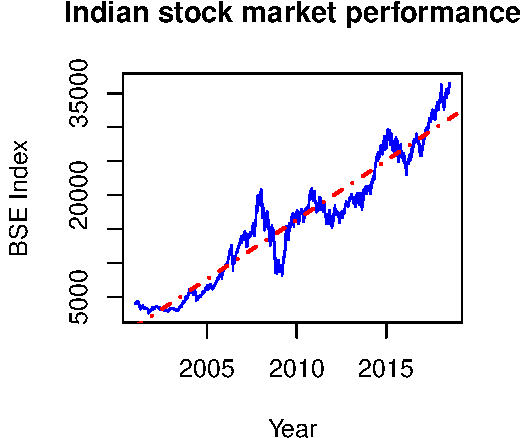
\includegraphics{FMC_T4_PhD_Fin_Time_Series_files/figure-latex/BSE-1} \end{center}

\begin{Shaded}
\begin{Highlighting}[]
\CommentTok{# via ggplot}

\KeywordTok{ggplot}\NormalTok{(}\DataTypeTok{data =}\NormalTok{ index_bse, }
       \KeywordTok{aes}\NormalTok{(Date, Close)}
\NormalTok{       ) }\OperatorTok{+}
\StringTok{  }\KeywordTok{geom_line}\NormalTok{(}\DataTypeTok{lwd =} \FloatTok{0.3}\NormalTok{,}
            \DataTypeTok{color =} \StringTok{"blue"}
\NormalTok{            ) }\OperatorTok{+}
\StringTok{  }\KeywordTok{geom_smooth}\NormalTok{(}\DataTypeTok{method =} \StringTok{"lm"}\NormalTok{,}
              \DataTypeTok{lty =} \StringTok{"dotdash"}\NormalTok{,}
              \DataTypeTok{lwd =} \FloatTok{0.6}\NormalTok{,}
              \DataTypeTok{color =} \StringTok{"red"}\NormalTok{,}
              \DataTypeTok{se =}\NormalTok{ F) }\OperatorTok{+}
\StringTok{  }\KeywordTok{theme_minimal}\NormalTok{() }\OperatorTok{+}
\StringTok{  }\KeywordTok{labs}\NormalTok{(}\DataTypeTok{x =} \StringTok{"Years"}\NormalTok{,}
       \DataTypeTok{y =} \StringTok{"BSE Sensex"}\NormalTok{,}
       \DataTypeTok{title =} \StringTok{"Indian stock market performance"}
\NormalTok{       )}
\end{Highlighting}
\end{Shaded}

\begin{center}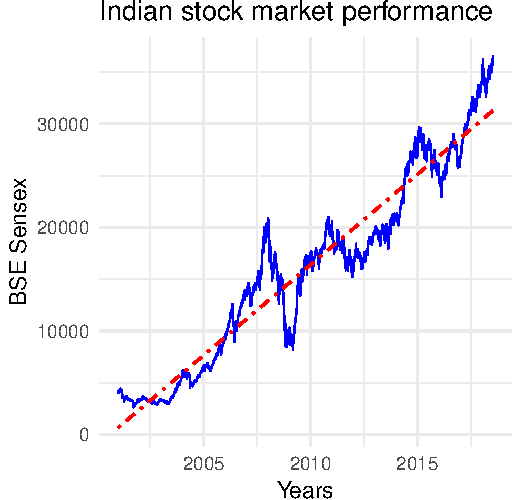
\includegraphics{FMC_T4_PhD_Fin_Time_Series_files/figure-latex/BSE-2} \end{center}

It seems that the level of the series is rising and the fluctuations are
sometimes high and sometimes low.

This index series is an example of a \emph{non-stationary} time series.
This roughly means that the mean and the variance of such a series are
functions of time.

Here is the index level time series for the US index S\&P500 from 2008:

\begin{Shaded}
\begin{Highlighting}[]
\NormalTok{file_sp500 <-}\StringTok{ "SP500.csv"} \CommentTok{#S&P 500}
\NormalTok{ind_sp500 <-}\StringTok{ }\NormalTok{readr}\OperatorTok{::}\KeywordTok{read_csv}\NormalTok{(file_sp500, }
                             \DataTypeTok{col_types =} \KeywordTok{cols}\NormalTok{(}\DataTypeTok{DATE =} \KeywordTok{col_date}\NormalTok{(), }
                                              \DataTypeTok{SP500 =} \KeywordTok{col_double}\NormalTok{()}
\NormalTok{                                              ),}
                             \DataTypeTok{na =} \KeywordTok{c}\NormalTok{(}\StringTok{""}\NormalTok{, }\StringTok{"NA"}\NormalTok{, }\StringTok{"."}\NormalTok{)}
\NormalTok{                             )}

\KeywordTok{ggplot}\NormalTok{(ind_sp500, }
       \KeywordTok{aes}\NormalTok{(DATE, SP500)}
\NormalTok{       ) }\OperatorTok{+}
\StringTok{  }\KeywordTok{geom_line}\NormalTok{(}\DataTypeTok{lwd =} \FloatTok{0.3}\NormalTok{,}
            \DataTypeTok{color =} \StringTok{"blue"}\NormalTok{) }\OperatorTok{+}
\StringTok{  }\KeywordTok{geom_smooth}\NormalTok{(}\DataTypeTok{method =} \StringTok{"lm"}\NormalTok{,}
              \DataTypeTok{lty =} \StringTok{"dotdash"}\NormalTok{,}
              \DataTypeTok{lwd =} \FloatTok{0.6}\NormalTok{,}
              \DataTypeTok{se =}\NormalTok{ F,}
              \DataTypeTok{color =} \StringTok{"red"}
\NormalTok{              ) }\OperatorTok{+}
\StringTok{  }\KeywordTok{theme_minimal}\NormalTok{() }\OperatorTok{+}
\StringTok{  }\KeywordTok{labs}\NormalTok{(}\DataTypeTok{x =} \StringTok{"Years"}\NormalTok{,}
       \DataTypeTok{y =} \StringTok{"S&P500"}
\NormalTok{       )}
\end{Highlighting}
\end{Shaded}

\begin{verbatim}
## Warning: Removed 92 rows containing non-finite values (stat_smooth).
\end{verbatim}

\begin{center}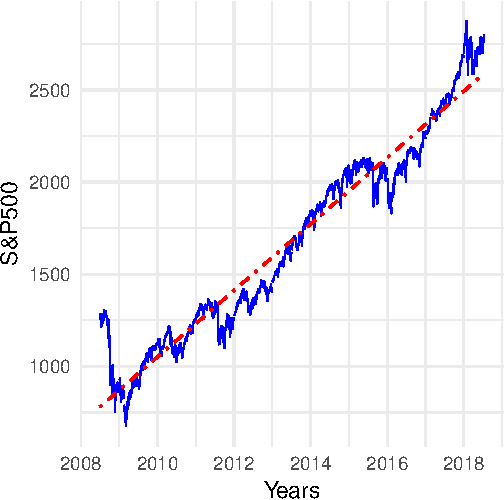
\includegraphics{FMC_T4_PhD_Fin_Time_Series_files/figure-latex/SP500-1} \end{center}

And here it for the Japanese Nikkei225:

\begin{Shaded}
\begin{Highlighting}[]
\NormalTok{file_nikkei <-}\StringTok{ "NIKKEI225.csv"} \CommentTok{#Nikkei 225}
\NormalTok{ind_nikkei <-}\StringTok{ }\NormalTok{readr}\OperatorTok{::}\KeywordTok{read_csv}\NormalTok{(file_nikkei, }
                             \DataTypeTok{col_types =} \KeywordTok{cols}\NormalTok{(}\DataTypeTok{DATE =} \KeywordTok{col_date}\NormalTok{(), }
                                              \DataTypeTok{NIKKEI225 =} \KeywordTok{col_double}\NormalTok{()}
\NormalTok{                                              ),}
                             \DataTypeTok{na =} \KeywordTok{c}\NormalTok{(}\StringTok{""}\NormalTok{, }\StringTok{"NA"}\NormalTok{, }\StringTok{"."}\NormalTok{)}
\NormalTok{                             )}

\KeywordTok{ggplot}\NormalTok{(ind_nikkei, }
       \KeywordTok{aes}\NormalTok{(DATE, NIKKEI225)}
\NormalTok{       ) }\OperatorTok{+}
\StringTok{  }\KeywordTok{geom_line}\NormalTok{(}\DataTypeTok{lwd =} \FloatTok{0.3}\NormalTok{, }
            \DataTypeTok{color =} \StringTok{"blue"}\NormalTok{) }\OperatorTok{+}
\StringTok{  }\KeywordTok{geom_smooth}\NormalTok{(}\DataTypeTok{method =} \StringTok{"lm"}\NormalTok{,}
              \DataTypeTok{lty =} \StringTok{"dotdash"}\NormalTok{,}
              \DataTypeTok{lwd =} \FloatTok{0.6}\NormalTok{,}
              \DataTypeTok{se =}\NormalTok{ F,}
              \DataTypeTok{color =} \StringTok{"red"}
\NormalTok{              ) }\OperatorTok{+}
\StringTok{  }\KeywordTok{theme_minimal}\NormalTok{() }\OperatorTok{+}
\StringTok{  }\KeywordTok{labs}\NormalTok{(}\DataTypeTok{x =} \StringTok{"Years"}\NormalTok{,}
       \DataTypeTok{y =} \StringTok{"Nikkei225"}
\NormalTok{       )}
\end{Highlighting}
\end{Shaded}

\begin{center}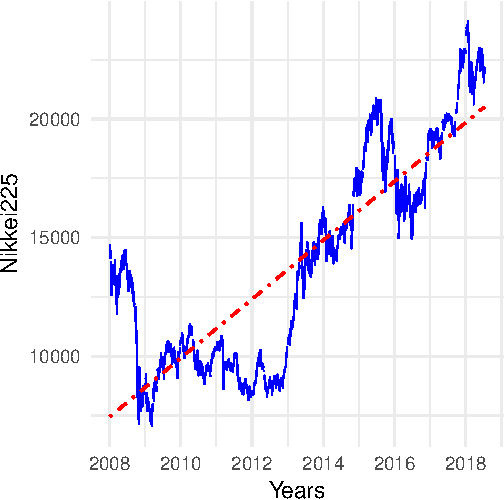
\includegraphics{FMC_T4_PhD_Fin_Time_Series_files/figure-latex/Nikkei-1} \end{center}

\section{Returns}\label{returns}

We observe prices in the financial markets empirically. However, due to
their non-stationary nature, they are hard to analyze. Hence they are
converted to return series which are usually stationary. There are many
ways to construct different notions of returns from the same underlying
price sequence. We discuss some prominent ones below.

\subsection{One-Period Simple Return}\label{one-period-simple-return}

The simple one period return for holding some asset whose price is given
by the sequence \(\{p_t\}_{t=1}^n\) is:

\[r_t := \frac{p_t-p_{t-1}}{p_{t-1}} = \frac{p_t}{p_{t-1}}-1\]

\subsection{Multi-period Simple
Return}\label{multi-period-simple-return}

\[r_t[k] := \frac{p_t-p_{t-k}}{p_{t-k}} = \frac{p_t}{p_{t-k}}-1\]
\[r_t[k] := \frac{p_t}{p_{t-k}}-1 = 
\frac{p_t}{p_{t-1}}\frac{p_{t-1}}{p_{t-2}}\hdots\frac{p_{t-k+1}}{p_{t-k}}-1\]
\[r_t[k] := (1+r_t)(1+r_{t-1})\hdots(1+r_{t-k+1})-1\]

Multi-period returns are used to convert high frequency returns to low
frequency returns---i.e., daily to monthly; or monthly to yearly etc.

For example to convert monthly returns to annual returns:
\[r_{t}[12]= [\prod_{j=0}^{12-1}(1+r_{t-j})]^{1/12}-1\]

Often (when working with daily returns especially) \(1+r_t\approx r_t\),
in which case: \[r_t[k]\approx \sum_{j=0}^{k-1}r_{t-j}\]

Additionally, the simple returns for a portfolio with fractional weights
\(w_1,\hdots,w_n\) are: \[r_{p,t}=\sum_{i=1}^n w_ir_{i,t}\]

\subsection{Log Returns}\label{log-returns}

We know that to compute yearly returns from say, monthly returns we use
the following formula:
\[r_{t}[12]= [\prod_{j=0}^{12-1}(1+r_{t-j})]^{1/12}-1\]

In general, if a bank pays an annual interest of \(r^m_t\) \(m\) times a
year, the interest rate for unit investment is \(r^m_t/m\) and after one
year the value of the deposit is \((1+\frac{r_t^m}{m})^m\). If there is
continous compounding, \(m\to \infty\), in which case the value of the
investment becomes:

\[\lim\limits_{m\to \infty}(1+\frac{r_t^m}{m})^m = e^{r_t}\]

Hence it must be that:
\[R_t = \log p_t-\log p_{t-1} = \log\frac{p_t}{p_{t-1}}\]

A particular advantage of log-returns are that multiperiod log returns
are merely the sum of one period log returns:

\[R_t[k]=\log p_t - \log p_{t-k}=\log p_t - \log p_{t-1} + \log p_{t-1} -\hdots \log p_{t-k}\]
\[R_t[k]= R_t[1]+R_t[2]+\hdots+R_t[k-1]\]

\subsection{Computational Examples}\label{computational-examples}

To construct return series from prices, we write a function that accepts
as input a price (or index) sequence and returns a sequence of simple
one period returns by using the formula
\(r_t = \frac{p_t-p_{t-1}}{p_{t-1}}\). Since there is no return for the
first entry of the price sequence, we append an \texttt{NA} at the
beginning of the returns.

\begin{Shaded}
\begin{Highlighting}[]
\NormalTok{func_pr_to_ret <-}\StringTok{ }\ControlFlowTok{function}\NormalTok{(price_vec)}
\NormalTok{\{}
  \CommentTok{# This function takes a vector of prices and }
  \CommentTok{# returns a vector of simple one period returns}
\NormalTok{  l <-}\StringTok{ }\KeywordTok{length}\NormalTok{(price_vec) }
\NormalTok{  ret_num <-}\StringTok{ }\KeywordTok{diff}\NormalTok{(price_vec) }\CommentTok{#numerator = change in prices}
\NormalTok{  ret_den <-}\StringTok{ }\NormalTok{price_vec[}\OperatorTok{-}\NormalTok{l] }\CommentTok{#denominator = price series}
  
  \KeywordTok{return}\NormalTok{(}\KeywordTok{c}\NormalTok{(}\OtherTok{NA}\NormalTok{, ret_num}\OperatorTok{/}\NormalTok{ret_den)) }\CommentTok{#first return is NA}
\NormalTok{\}}

\NormalTok{price_vec_}\DecValTok{1}\NormalTok{ <-}\StringTok{ }\KeywordTok{seq}\NormalTok{(}\DataTypeTok{from =} \DecValTok{1}\NormalTok{, }\DataTypeTok{to =} \DecValTok{10}\NormalTok{, }\DataTypeTok{by =} \DecValTok{2}\NormalTok{)}
\KeywordTok{func_pr_to_ret}\NormalTok{(price_vec_}\DecValTok{1}\NormalTok{)}
\end{Highlighting}
\end{Shaded}

\begin{verbatim}
## [1]        NA 2.0000000 0.6666667 0.4000000 0.2857143
\end{verbatim}

Similarly log-returns can be calculated using the formuala
\(R_t = \log(p_t)-\log(p_{t-1})\).

\begin{Shaded}
\begin{Highlighting}[]
\NormalTok{func_pr_to_logret <-}\StringTok{ }\ControlFlowTok{function}\NormalTok{(p_vec)}
\NormalTok{\{}
  \CommentTok{# This function takes a vector of prices and }
  \CommentTok{# returns a vector of log returns}
\NormalTok{  log_price <-}\StringTok{ }\KeywordTok{log}\NormalTok{(p_vec)}
\NormalTok{  log_ret <-}\StringTok{ }\KeywordTok{diff}\NormalTok{(log_price) }\CommentTok{#log ret = delta log p}
  
  \KeywordTok{return}\NormalTok{(}\KeywordTok{c}\NormalTok{(}\OtherTok{NA}\NormalTok{, log_ret)) }\CommentTok{#first return is NA}
\NormalTok{\}}

\NormalTok{p_vec <-}\StringTok{ }\KeywordTok{seq}\NormalTok{(}\DataTypeTok{from =} \DecValTok{1}\NormalTok{, }\DataTypeTok{to =} \DecValTok{10}\NormalTok{, }\DataTypeTok{by =} \DecValTok{2}\NormalTok{)}
\KeywordTok{func_pr_to_logret}\NormalTok{(p_vec)}
\end{Highlighting}
\end{Shaded}

\begin{verbatim}
## [1]        NA 1.0986123 0.5108256 0.3364722 0.2513144
\end{verbatim}

\subsection{Return Series for Market
Indices}\label{return-series-for-market-indices}

We can compute returns and log-returns for the Bombay Stock Exchange
Index, S\&P500 and the Nikkei 225 as follows:

\begin{Shaded}
\begin{Highlighting}[]
\NormalTok{ret_BSE <-}\StringTok{ }\KeywordTok{func_pr_to_ret}\NormalTok{(index_bse}\OperatorTok{$}\NormalTok{Close)}
\KeywordTok{plot}\NormalTok{(index_bse}\OperatorTok{$}\NormalTok{Date, }\CommentTok{#x variable}
\NormalTok{     ret_BSE, }\CommentTok{#y variable}
     \DataTypeTok{type =} \StringTok{"l"}\NormalTok{,}
     \DataTypeTok{lwd =} \FloatTok{1.2}\NormalTok{,}
     \DataTypeTok{col =} \StringTok{"blue"}\NormalTok{,}
     \DataTypeTok{xlab =} \StringTok{"Years"}\NormalTok{,}
     \DataTypeTok{ylab =} \StringTok{"BSE Returns"}
\NormalTok{     )}
\KeywordTok{abline}\NormalTok{(}\DataTypeTok{h =} \DecValTok{0}\NormalTok{)}
\end{Highlighting}
\end{Shaded}

\begin{center}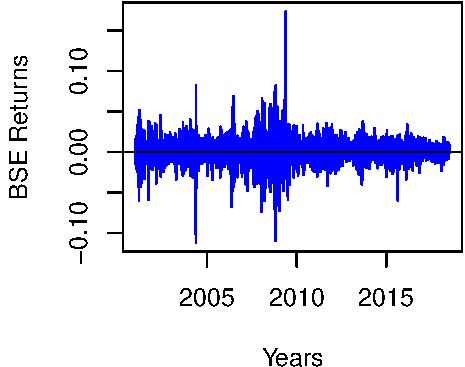
\includegraphics{FMC_T4_PhD_Fin_Time_Series_files/figure-latex/return_market_index-1} \end{center}

We can do the same for the S\&P500 and the Nikkei225 series:

\begin{Shaded}
\begin{Highlighting}[]
\NormalTok{ret_sp500 <-}\StringTok{ }\KeywordTok{func_pr_to_ret}\NormalTok{(ind_sp500}\OperatorTok{$}\NormalTok{SP500)}
\KeywordTok{plot}\NormalTok{(ind_sp500}\OperatorTok{$}\NormalTok{DATE, }\CommentTok{#x variable}
\NormalTok{     ret_sp500, }\CommentTok{#y variable}
     \DataTypeTok{type =} \StringTok{"l"}\NormalTok{,}
     \DataTypeTok{lwd =} \FloatTok{1.2}\NormalTok{,}
     \DataTypeTok{col =} \StringTok{"red"}\NormalTok{,}
     \DataTypeTok{xlab =} \StringTok{"Years"}\NormalTok{,}
     \DataTypeTok{ylab =} \StringTok{"S&P500 Returns"}
\NormalTok{     )}
\KeywordTok{abline}\NormalTok{(}\DataTypeTok{h =} \DecValTok{0}\NormalTok{)}
\end{Highlighting}
\end{Shaded}

\begin{center}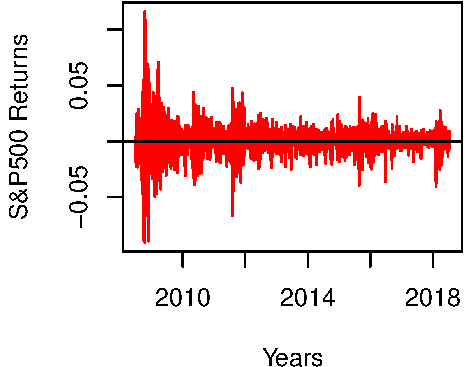
\includegraphics{FMC_T4_PhD_Fin_Time_Series_files/figure-latex/return_market_index_func-1} \end{center}

\begin{Shaded}
\begin{Highlighting}[]
\NormalTok{ret_nikkei <-}\StringTok{ }\KeywordTok{func_pr_to_ret}\NormalTok{(ind_nikkei}\OperatorTok{$}\NormalTok{NIKKEI225)}
\KeywordTok{plot}\NormalTok{(ind_nikkei}\OperatorTok{$}\NormalTok{DATE, }\CommentTok{#x variable}
\NormalTok{     ret_nikkei, }\CommentTok{#y variable}
     \DataTypeTok{type =} \StringTok{"l"}\NormalTok{,}
     \DataTypeTok{lwd =} \FloatTok{1.2}\NormalTok{,}
     \DataTypeTok{col =} \StringTok{"green"}\NormalTok{,}
     \DataTypeTok{xlab =} \StringTok{"Years"}\NormalTok{,}
     \DataTypeTok{ylab =} \StringTok{"Nikkei225 Returns"}
\NormalTok{     )}
\KeywordTok{abline}\NormalTok{(}\DataTypeTok{h =} \DecValTok{0}\NormalTok{)}
\end{Highlighting}
\end{Shaded}

\begin{center}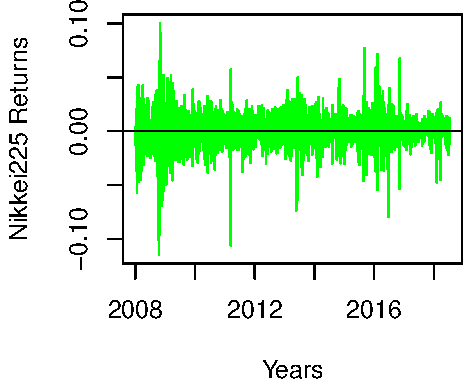
\includegraphics{FMC_T4_PhD_Fin_Time_Series_files/figure-latex/return_market_index_func-2} \end{center}

One clearly sees that the index sequences have no trend now. It seems
that the returns are fluctuating around a mean level 0. The fluctuations
(volatility) around the mean are sometimes high and sometimes low.

\section{Stationarity of Time Series}\label{stationarity-of-time-series}

There's a clear difference between the plots of prices (or indices like
the BSE); and the returns derived from them. Indices keep increasing
with time, suggesting some type of a trend and tend to fluctuate more or
less around the trend line. Returns, on the other hand seem to have no
trend.

\subsection{Stationarity}\label{stationarity}

A (strictly) \emph{stationary} process is one for which the
unconditional joint distribution does not change with time:
\[F_X(x_1,\hdots,x_t)=F_X(x_{1+\delta},\hdots,x_{t+\delta})\]

where \(F_X(\cdot)\) is the distribution for the process \(X_t\) and
\(\delta>0\).

In particular this implies that the mean and the variance (and other
central moments) do not change with time.

Inference for nonstationary series is difficult. Hence in practice we
convert nonstationary processes to stationary processes before analyzing
them.

A \emph{weakly stationary} time series is such that the mean of the
process \(\mathbb{E}(X_t) = \mu(t) = \mu\) and its (auto)covariance
\(\text{covar}(X_t, X_{t-\delta}) = \sigma_{\delta}\) depends only on
the lag \(\delta\).

Strictly stationary series are weakly stationary but not vice versa.

\subsubsection{Trend Stationarity}\label{trend-stationarity}

If the trend (mean) of the nonstationary process is deterministic, we
have trend stationarity: \[X_t = \mu(t) + \epsilon_t\]

where \(\mu(\cdot)\) is a real function and \(\epsilon_t\) is stationary
process (say, \(\mathcal{N}(0,1)\)).

Here is an illustration---suppose the mean is \(\mu(t) = 1 + 2t\):

\begin{Shaded}
\begin{Highlighting}[]
\NormalTok{t <-}\StringTok{ }\KeywordTok{seq}\NormalTok{(}\DecValTok{0}\NormalTok{, }\DecValTok{100}\NormalTok{, }\FloatTok{0.4}\NormalTok{)}

\KeywordTok{plot}\NormalTok{((}\DecValTok{1} \OperatorTok{+}\StringTok{ }\DecValTok{2}\OperatorTok{*}\NormalTok{t }\OperatorTok{+}\StringTok{ }\KeywordTok{rnorm}\NormalTok{(}\KeywordTok{length}\NormalTok{(t), }\DecValTok{0}\NormalTok{, }\DecValTok{10}\NormalTok{)),}
     \DataTypeTok{type =} \StringTok{"l"}\NormalTok{,}
     \DataTypeTok{lwd =} \DecValTok{2}\NormalTok{,}
     \DataTypeTok{col =} \StringTok{"green"}\NormalTok{,}
     \DataTypeTok{xlab =} \StringTok{"index"}\NormalTok{,}
     \DataTypeTok{main =} \StringTok{"Trend stationary seris"}
\NormalTok{     )}
\KeywordTok{lines}\NormalTok{((}\DecValTok{1}\OperatorTok{+}\DecValTok{2}\OperatorTok{*}\NormalTok{t),}
      \DataTypeTok{type =} \StringTok{"l"}\NormalTok{,}
      \DataTypeTok{col =} \StringTok{"red"}\NormalTok{,}
      \DataTypeTok{lty =} \StringTok{"dotdash"}\NormalTok{,}
      \DataTypeTok{lwd =} \FloatTok{1.2}
\NormalTok{      )}
\end{Highlighting}
\end{Shaded}

\begin{center}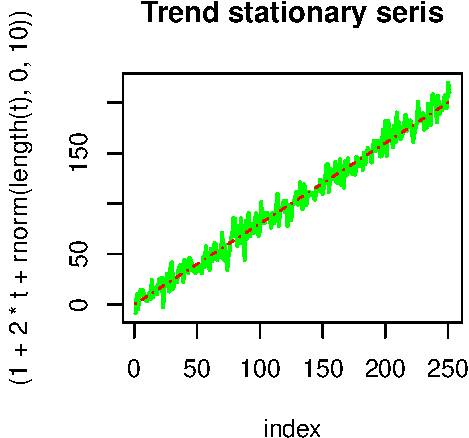
\includegraphics{FMC_T4_PhD_Fin_Time_Series_files/figure-latex/trend_stationary-1} \end{center}

This can be made into a stationary process by \emph{detrending}:
subtracting \(\mu(t) = 1+2t\) from the series, to recover
\(X_t-\mu(t)=\epsilon_t\sim \mathcal{N}(0, 10)\) in this case:

\begin{Shaded}
\begin{Highlighting}[]
\KeywordTok{plot}\NormalTok{((}\DecValTok{1} \OperatorTok{+}\StringTok{ }\DecValTok{2}\OperatorTok{*}\NormalTok{t }\OperatorTok{+}\StringTok{ }\KeywordTok{rnorm}\NormalTok{(}\KeywordTok{length}\NormalTok{(t), }\DecValTok{0}\NormalTok{, }\DecValTok{10}\NormalTok{) }\OperatorTok{-}\StringTok{ }\NormalTok{(}\DecValTok{1} \OperatorTok{+}\StringTok{ }\DecValTok{2}\OperatorTok{*}\NormalTok{t)),}
     \DataTypeTok{type =} \StringTok{"l"}\NormalTok{,}
     \DataTypeTok{main =} \StringTok{"Detrended series"}\NormalTok{,}
     \DataTypeTok{col =} \StringTok{"green"}
\NormalTok{     )}
\KeywordTok{abline}\NormalTok{(}\DataTypeTok{h =} \DecValTok{0}\NormalTok{)}
\end{Highlighting}
\end{Shaded}

\begin{center}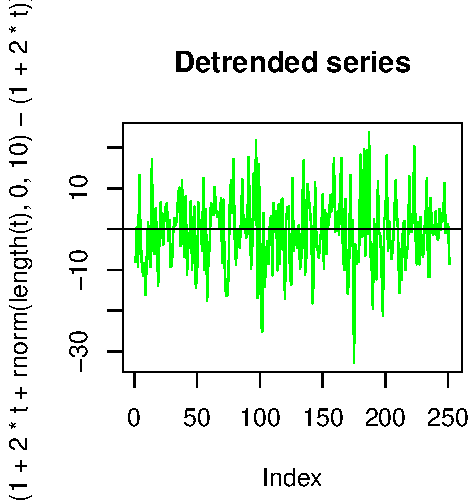
\includegraphics{FMC_T4_PhD_Fin_Time_Series_files/figure-latex/detrend-1} \end{center}

Additionally trend stationary series are \emph{mean-reverting} which
means that after encountering an exogenous shock they tend to revert to
the fluctuations-around-the-mean behavior.

\subsubsection{Unit Roots}\label{unit-roots}

A stochastic process has a unit root if 1 is the root of its
characteristic equation. For example consider the following process:

\[X_t = X_{t-1} + \epsilon_t\]

It's characteristic equation is: \(x - 1 = 0\). It's clear that
\(X_t - X_{t-1} = \epsilon_t\) is a stationary process.

Note that for trend stationary series we \emph{detrended} to obtain a
stationary series while for a unit root process, we
\emph{first-differenced} to arrive at a stationary series. Random walks
are examples of unit root processes.

By repeated additions:

\[X_T = X_0 + \sum_{t = 1}^T \epsilon_t\]

Hence \(\mathbb{E}(X_T) = X_0 + \mathbb{E}(\epsilon_T) = X_0\); and
\(\text{var}(X_T) = \text{var}(\sum_{t = 1}^T \epsilon_t) = T\cdot \sigma^2\).

\begin{Shaded}
\begin{Highlighting}[]
\KeywordTok{plot}\NormalTok{(}\KeywordTok{cumsum}\NormalTok{(}\KeywordTok{rnorm}\NormalTok{(}\DecValTok{1000}\NormalTok{, }\DecValTok{0}\NormalTok{, }\DecValTok{10}\NormalTok{)),}
     \DataTypeTok{type =} \StringTok{"l"}\NormalTok{,}
     \DataTypeTok{lwd =} \FloatTok{1.5}\NormalTok{,}
     \DataTypeTok{col =} \StringTok{"red"}\NormalTok{,}
     \DataTypeTok{main =} \StringTok{"Unit root process"}
\NormalTok{     )}
\end{Highlighting}
\end{Shaded}

\begin{center}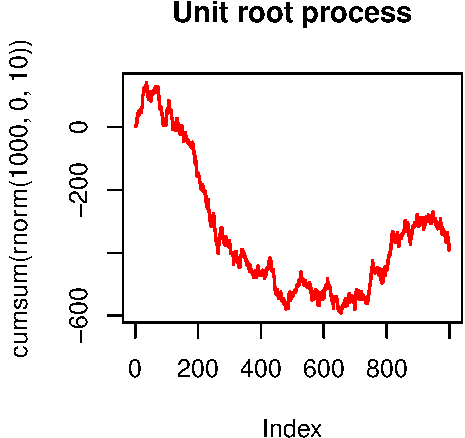
\includegraphics{FMC_T4_PhD_Fin_Time_Series_files/figure-latex/unit_root-1} \end{center}

\begin{Shaded}
\begin{Highlighting}[]
\KeywordTok{plot}\NormalTok{(}\KeywordTok{rnorm}\NormalTok{(}\DecValTok{1000}\NormalTok{, }\DecValTok{0}\NormalTok{, }\DecValTok{10}\NormalTok{),}
     \DataTypeTok{type =} \StringTok{"l"}\NormalTok{,}
     \DataTypeTok{col =} \StringTok{"blue"}\NormalTok{,}
     \DataTypeTok{main =} \StringTok{"Differenced unit root process"}
\NormalTok{     )}
\end{Highlighting}
\end{Shaded}

\begin{center}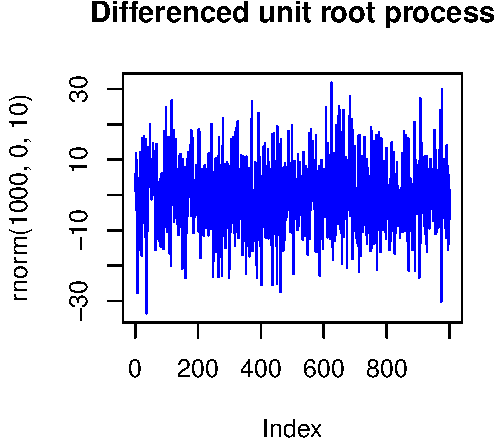
\includegraphics{FMC_T4_PhD_Fin_Time_Series_files/figure-latex/unit_root-2} \end{center}

Unit root processes are not mean reverting---an exogenous shock can
permanently alter the behavior of the unit root process.

\section{Distribution of Returns}\label{distribution-of-returns}

Are all return values for the indices considered above equally likely to
occur? If that is the case, the returns will be uniformly distributed. A
quick glance at the figures however suggests that perhaps some other
distribution ought to be considered.

\subsection{Summary Statistics of Empirical
Returns}\label{summary-statistics-of-empirical-returns}

For the three indices and their return series considered above (the BSE
Sensex, the S\&P500, the Nikkei225) we compute summary statistics below:

\begin{Shaded}
\begin{Highlighting}[]
\NormalTok{func_summ_stat_ind <-}\StringTok{ }\ControlFlowTok{function}\NormalTok{(vec)}
\NormalTok{\{}
\NormalTok{  summ_stat_ind <-}\StringTok{ }\KeywordTok{data.frame}\NormalTok{(}\DataTypeTok{min =} \KeywordTok{min}\NormalTok{(vec, }\DataTypeTok{na.rm =}\NormalTok{ T),}
                       \DataTypeTok{max =} \KeywordTok{max}\NormalTok{(vec, }\DataTypeTok{na.rm =}\NormalTok{ T),}
                       \DataTypeTok{mean =} \KeywordTok{mean}\NormalTok{(vec, }\DataTypeTok{na.rm =}\NormalTok{ T),}
                       \DataTypeTok{median =} \KeywordTok{median}\NormalTok{(vec, }\DataTypeTok{na.rm =}\NormalTok{T),}
                       \DataTypeTok{std =} \KeywordTok{sd}\NormalTok{(vec, }\DataTypeTok{na.rm =}\NormalTok{T),}
                       \DataTypeTok{iqr =} \KeywordTok{IQR}\NormalTok{(vec, }\DataTypeTok{na.rm=}\NormalTok{T),}
                       \DataTypeTok{var =} \KeywordTok{var}\NormalTok{(vec, }\DataTypeTok{na.rm =}\NormalTok{T)}
\NormalTok{                       ) }\OperatorTok
\StringTok{    }\KeywordTok{signif}\NormalTok{(., }\DataTypeTok{digits =} \DecValTok{2}\NormalTok{) }\CommentTok{#significant digits = 2}
  
  \KeywordTok{return}\NormalTok{(summ_stat_ind)}

\NormalTok{\}}

\NormalTok{table_summ_stat <-}\StringTok{ }\KeywordTok{rbind}\NormalTok{(}\KeywordTok{c}\NormalTok{(}\StringTok{"BSE"}\NormalTok{, }\KeywordTok{func_summ_stat_ind}\NormalTok{(ret_BSE)), }
                         \KeywordTok{c}\NormalTok{(}\StringTok{"S&P500"}\NormalTok{, }\KeywordTok{func_summ_stat_ind}\NormalTok{(ret_sp500)), }
                         \KeywordTok{c}\NormalTok{(}\StringTok{"Nikkei225"}\NormalTok{, }\KeywordTok{func_summ_stat_ind}\NormalTok{(ret_nikkei))}
\NormalTok{                         )}

\NormalTok{knitr}\OperatorTok{::}\KeywordTok{kable}\NormalTok{(table_summ_stat)}
\end{Highlighting}
\end{Shaded}

\begin{longtable}[]{@{}llllllll@{}}
\toprule
& min & max & mean & median & std & iqr & var\tabularnewline
\midrule
\endhead
BSE & -0.11 & 0.17 & 0.00061 & 0.00092 & 0.014 & 0.014 &
2e-04\tabularnewline
S\&P500 & -0.09 & 0.12 & 0.00038 & 0.00061 & 0.013 & 0.0093 &
0.00016\tabularnewline
Nikkei225 & -0.11 & 0.1 & 0.00014 & 0.00059 & 0.016 & 0.015 &
0.00024\tabularnewline
\bottomrule
\end{longtable}

For all series, the medians are about 1.5--3 times the corresponding
means. This suggests that there are significant negative outliers.

In general though, a natural choice for modeling return distribution is
the ubiquitous normal distribution. To check if it is a plausible
candidate, we plot the empirical histogram of returns for all three
series separately.

\subsection{Histograms for returns for each
index}\label{histograms-for-returns-for-each-index}

\begin{Shaded}
\begin{Highlighting}[]
\KeywordTok{hist}\NormalTok{(ret_BSE,}
     \DataTypeTok{breaks =} \DecValTok{80}\NormalTok{,}
     \DataTypeTok{col =} \StringTok{"grey"}\NormalTok{,}
     \DataTypeTok{xlab =} \StringTok{"Daily Returns"}\NormalTok{,}
     \DataTypeTok{ylab =} \StringTok{"Frequency"}\NormalTok{,}
     \DataTypeTok{main =} \StringTok{"Histogram for BSE"}
\NormalTok{     )}
\end{Highlighting}
\end{Shaded}

\begin{center}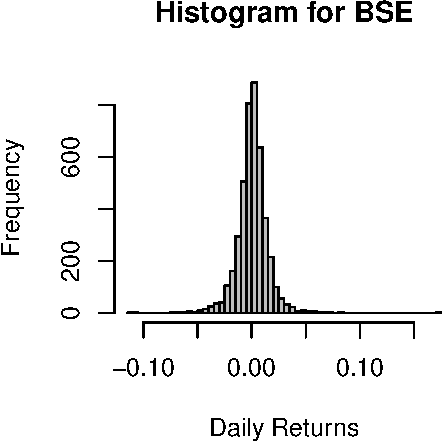
\includegraphics{FMC_T4_PhD_Fin_Time_Series_files/figure-latex/histograms-1} \end{center}

\begin{Shaded}
\begin{Highlighting}[]
\KeywordTok{hist}\NormalTok{(ret_sp500,}
     \DataTypeTok{breaks =} \DecValTok{80}\NormalTok{,}
     \DataTypeTok{col =} \StringTok{"grey"}\NormalTok{,}
     \DataTypeTok{xlab =} \StringTok{"Daily Returns"}\NormalTok{,}
     \DataTypeTok{ylab =} \StringTok{"Frequency"}\NormalTok{,}
     \DataTypeTok{main =} \StringTok{"Histogram for S&P500"}
\NormalTok{     )}
\end{Highlighting}
\end{Shaded}

\begin{center}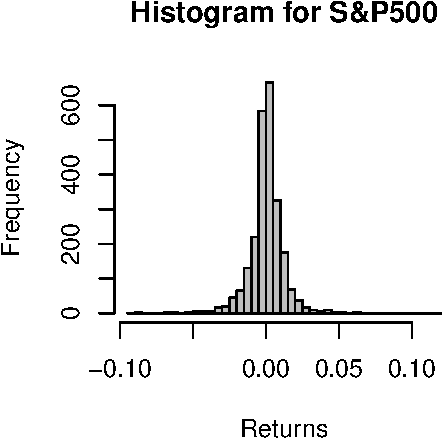
\includegraphics{FMC_T4_PhD_Fin_Time_Series_files/figure-latex/histograms-2} \end{center}

\begin{Shaded}
\begin{Highlighting}[]
\KeywordTok{hist}\NormalTok{(ret_nikkei,}
     \DataTypeTok{breaks =} \DecValTok{80}\NormalTok{,}
     \DataTypeTok{col =} \StringTok{"grey"}\NormalTok{,}
     \DataTypeTok{xlab =} \StringTok{"Daily Returns"}\NormalTok{,}
     \DataTypeTok{ylab =} \StringTok{"Frequency"}\NormalTok{,}
     \DataTypeTok{main =} \StringTok{"Histogram for Nikkei225"}
\NormalTok{     )}
\end{Highlighting}
\end{Shaded}

\begin{center}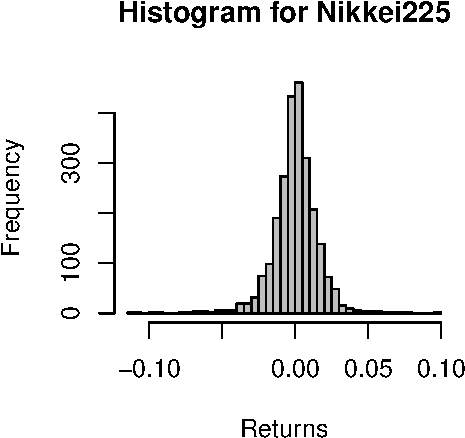
\includegraphics{FMC_T4_PhD_Fin_Time_Series_files/figure-latex/histograms-3} \end{center}

The three histograms do resemble a normal density. All of them display
the classic bell curve characteristics. However, merely eyeballing the
data is not proof enough.

\subsubsection{Skewness and Kurtosis}\label{skewness-and-kurtosis}

One way to test if the data are normally distributed is to check their
third and fourth central moments---the skewness and kurtosis. For normal
random variables, the skewness must be 0 (the bell curve is unimodal and
symmetric about its mean); and the kurtosis must be 3. If the data
display substantial departures from such values there may be evidence of
non-normality.

Formally the skewness and kurtosis are defined as:

\[s = \mathbb{E}(\frac{X-\mu}{\sigma})^3\]
\[\kappa = \mathbb{E}(\frac{X-\mu}{\sigma})^4\]

We compute the skewness and kurtosis of the return series for the three
indices as follows:

\begin{Shaded}
\begin{Highlighting}[]
\NormalTok{skew <-}\StringTok{ }\KeywordTok{rbind}\NormalTok{(moments}\OperatorTok{::}\KeywordTok{skewness}\NormalTok{(ret_BSE, }\DataTypeTok{na.rm =}\NormalTok{ T),}
\NormalTok{              moments}\OperatorTok{::}\KeywordTok{skewness}\NormalTok{(ret_sp500, }\DataTypeTok{na.rm =}\NormalTok{ T),}
\NormalTok{              moments}\OperatorTok{::}\KeywordTok{skewness}\NormalTok{(ret_nikkei, }\DataTypeTok{na.rm =}\NormalTok{ T)}
\NormalTok{              )}

\NormalTok{kurt <-}\StringTok{ }\KeywordTok{rbind}\NormalTok{(moments}\OperatorTok{::}\KeywordTok{kurtosis}\NormalTok{(ret_BSE, }\DataTypeTok{na.rm =}\NormalTok{ T),}
\NormalTok{              moments}\OperatorTok{::}\KeywordTok{kurtosis}\NormalTok{(ret_sp500, }\DataTypeTok{na.rm =}\NormalTok{ T),}
\NormalTok{              moments}\OperatorTok{::}\KeywordTok{kurtosis}\NormalTok{(ret_nikkei, }\DataTypeTok{na.rm =}\NormalTok{ T)}
\NormalTok{              )}

\NormalTok{table_skew_kurt <-}\StringTok{ }\KeywordTok{data.frame}\NormalTok{(}\DataTypeTok{Skew =}\NormalTok{ skew, }
                              \DataTypeTok{Kurt =}\NormalTok{ kurt,}
                              \DataTypeTok{Excess_Kurt =}\NormalTok{ kurt}\OperatorTok{-}\DecValTok{3}
\NormalTok{                              )}

\NormalTok{knitr}\OperatorTok{::}\KeywordTok{kable}\NormalTok{(table_skew_kurt)}
\end{Highlighting}
\end{Shaded}

\begin{longtable}[]{@{}rrr@{}}
\toprule
Skew & Kurt & Excess\_Kurt\tabularnewline
\midrule
\endhead
0.0967129 & 12.870632 & 9.870632\tabularnewline
-0.0938530 & 15.121463 & 12.121463\tabularnewline
-0.6276185 & 9.691047 & 6.691047\tabularnewline
\bottomrule
\end{longtable}

There is substantial evidence from the table above to suggest that the
returns may be \emph{non-normal}. Formally however, we resort the
\emph{Jarque-Bera Test} to confirm our hypothesis.

\subsubsection{The Jarque-Bera Test for
Normality}\label{the-jarque-bera-test-for-normality}

There is a large literature that suggests two empirical regularities for
asset returns:

\begin{enumerate}
\def\labelenumi{\arabic{enumi}.}
\tightlist
\item
  Crashes occur more frequently than booms
\item
  Extreme events occur more frequently than suggested by normal
  distributions
\end{enumerate}

The first outcome is consistent with a distribution displaying
\emph{negative} skewness. The second outcome suggests \emph{excess
kurtosis}.

The Jarcque-Bera test is a moment based test that relis on the
observation that for a normal random variable the skewness and excess
kurtosis are both 0. The estimators for skewness and kurtosis are:
\[\hat{s} = \frac{1}{T}\sum_{t=1}^T (\frac{x_t-\bar{x}}{\hat{\sigma}})^3\]
\[\hat{\kappa} = \frac{1}{T}\sum_{t=1}^T (\frac{x_t-\bar{x}}{\hat{\sigma}})^4\]

and as \(T\to \infty\)

\[\sqrt T\cdot \hat{s} \to \mathcal{N}(0, 6)\]
\[\sqrt T\cdot (\hat{\kappa}-3) \to \mathcal{N}(0, 24)\]

Hence, for normal random variables

\[\frac{\hat{s}}{\sqrt(\frac{6}{T})}\to \mathcal{N}(0,1)\]
\[\frac{\hat{\kappa}-3}{\sqrt(\frac{24}{T})}\to \mathcal{N}(0,1)\]

The Jarque-Bera test statistic uses the following insight:

\[JB = T[\frac{\hat{s}^2}{6}+\frac{\hat{\kappa}-3}{24}]\to \chi^2(2)\]

In order to test if the returns from the three indices do follow the
normal distribution we employ the package \texttt{tseries} and the
function \texttt{jarque.bera.test()} in it. Note that it disallows any
\texttt{NA} values.

\begin{Shaded}
\begin{Highlighting}[]
\NormalTok{tseries}\OperatorTok{::}\KeywordTok{jarque.bera.test}\NormalTok{(}\KeywordTok{rnorm}\NormalTok{(}\DecValTok{1000}\NormalTok{, }\DecValTok{0}\NormalTok{, }\DecValTok{10}\NormalTok{)) }\CommentTok{#benchmarking}
\end{Highlighting}
\end{Shaded}

\begin{verbatim}
## 
##  Jarque Bera Test
## 
## data:  rnorm(1000, 0, 10)
## X-squared = 0.70629, df = 2, p-value = 0.7025
\end{verbatim}

\begin{Shaded}
\begin{Highlighting}[]
\NormalTok{tseries}\OperatorTok{::}\KeywordTok{jarque.bera.test}\NormalTok{(}\OperatorTok{!}\KeywordTok{is.na}\NormalTok{(ret_BSE)) }\CommentTok{#note: !is.na()}
\end{Highlighting}
\end{Shaded}

\begin{verbatim}
## 
##  Jarque Bera Test
## 
## data:  !is.na(ret_BSE)
## X-squared = 3465300000, df = 2, p-value < 2.2e-16
\end{verbatim}

\begin{Shaded}
\begin{Highlighting}[]
\NormalTok{tseries}\OperatorTok{::}\KeywordTok{jarque.bera.test}\NormalTok{(}\OperatorTok{!}\KeywordTok{is.na}\NormalTok{(ret_sp500))}
\end{Highlighting}
\end{Shaded}

\begin{verbatim}
## 
##  Jarque Bera Test
## 
## data:  !is.na(ret_sp500)
## X-squared = 14394, df = 2, p-value < 2.2e-16
\end{verbatim}

\begin{Shaded}
\begin{Highlighting}[]
\NormalTok{tseries}\OperatorTok{::}\KeywordTok{jarque.bera.test}\NormalTok{(}\OperatorTok{!}\KeywordTok{is.na}\NormalTok{(ret_nikkei))}
\end{Highlighting}
\end{Shaded}

\begin{verbatim}
## 
##  Jarque Bera Test
## 
## data:  !is.na(ret_nikkei)
## X-squared = 5265.2, df = 2, p-value < 2.2e-16
\end{verbatim}

\section{Stylized Facts}\label{stylized-facts}

Stock prices, commodity prices, exchange rates etc. in empirical
financial markets display many striking regularities discussed in Cont
(2001).

\begin{enumerate}
\def\labelenumi{\arabic{enumi}.}
\tightlist
\item
  \textbf{Fat Tails:} Unconditional return distributions have tails
  fatter than those of normal distribution. Conditional return
  distributions are also non-normal.
\item
  \textbf{Asymmetry:} Unconditional return distributions are negatively
  skewed.
\item
  \textbf{Aggregated Normality:} Lower frequency returns resemble normal
  distributions more than higher frequency returns.
\item
  \textbf{No Autocorrelation:} Except at high frequencies, returns
  generally do not display autocorrelation.
\item
  \textbf{Volatility Clustering:} Return volatility is autocorrelated.
\item
  \textbf{Time-Varying Cross Correlation:} Correlation between assets
  returns tends to be higher during high volatility periods especially
  during market crashes.
\end{enumerate}

\section*{References}\label{references}
\addcontentsline{toc}{section}{References}

\hypertarget{refs}{}
\hypertarget{ref-Cont:2001}{}
Cont, Rama. 2001. ``Empirical Properties of Asset Returns: Stylized
Facts and Statistical Issues.'' \emph{Quantitative Finance} 1 (2):
223--36.

\hypertarget{ref-Jondeau_Poon_Rockinger:2007}{}
Jondeau, Eric, Ser-Huang Poon, and Michael Rockinger. 2007.
\emph{Financial Modeling Under Non-Gaussian Distributions}. Springer
Finance.

\hypertarget{ref-Tsay:2010}{}
Tsay, Ruey S. 2010. \emph{Analysis of Financial Time Series}. Third
Edition. John Wiley; Sons.


\end{document}
